\documentclass{article}

\usepackage{amsmath}
\usepackage{graphicx}
\usepackage{listings}
\graphicspath{ {graphs/} }

\title{2XB3 Lab3}
\author{
  Yi Luo\\
  \texttt{400254211}\\
  \texttt{luoy94@mcmaster.ca}\\
  \texttt{L02}
  \and
  Frank Yang\\
  \texttt{400243777}\\
  \texttt{yangf51@mcmaster.ca}\\
  \texttt{L02}
  \and
  Harrison Chiu\\
  \texttt{400261400}\\
  \texttt{chiuh@mcmaster.ca}\\
  \texttt{L02}
}
\date{\today}

\begin{document}

\maketitle

\begin{abstract}
This paper analyzes different time complexities of quicksort. Specifically it looks into the time complexities of various quicksort implementations, including multiple pivots, different pivots, small lists, and worst case performance.
\end{abstract}

\section*{Quicksort Inplace}


\section*{Quicksort Multi-pivot}

\section*{Worst case}
The worst complexity of quicksort is $n^2$. It happens under the following 
circumstances. The given array is already sorted or reversely sorted with 
the leftmost or the rightmost element chosen as the pivot. The given array’s 
elements are the same.

All of them would lead to a situation where the divided arrays are totally 
unbalanced such that one array has only one element while the other has $n - 1$ 
element with $n$ being the size of the parental array. As a result, the time 
complexity would be as such:
\begin{equation*}
n + (n - 1) + (n - 2) + (n - 3) + … + 2 = n * (n + 1) / 2 – 1 = \Theta{n^2}
\end{equation*}

A graph is attached showing the average case performance vs the worst case performance vs n.

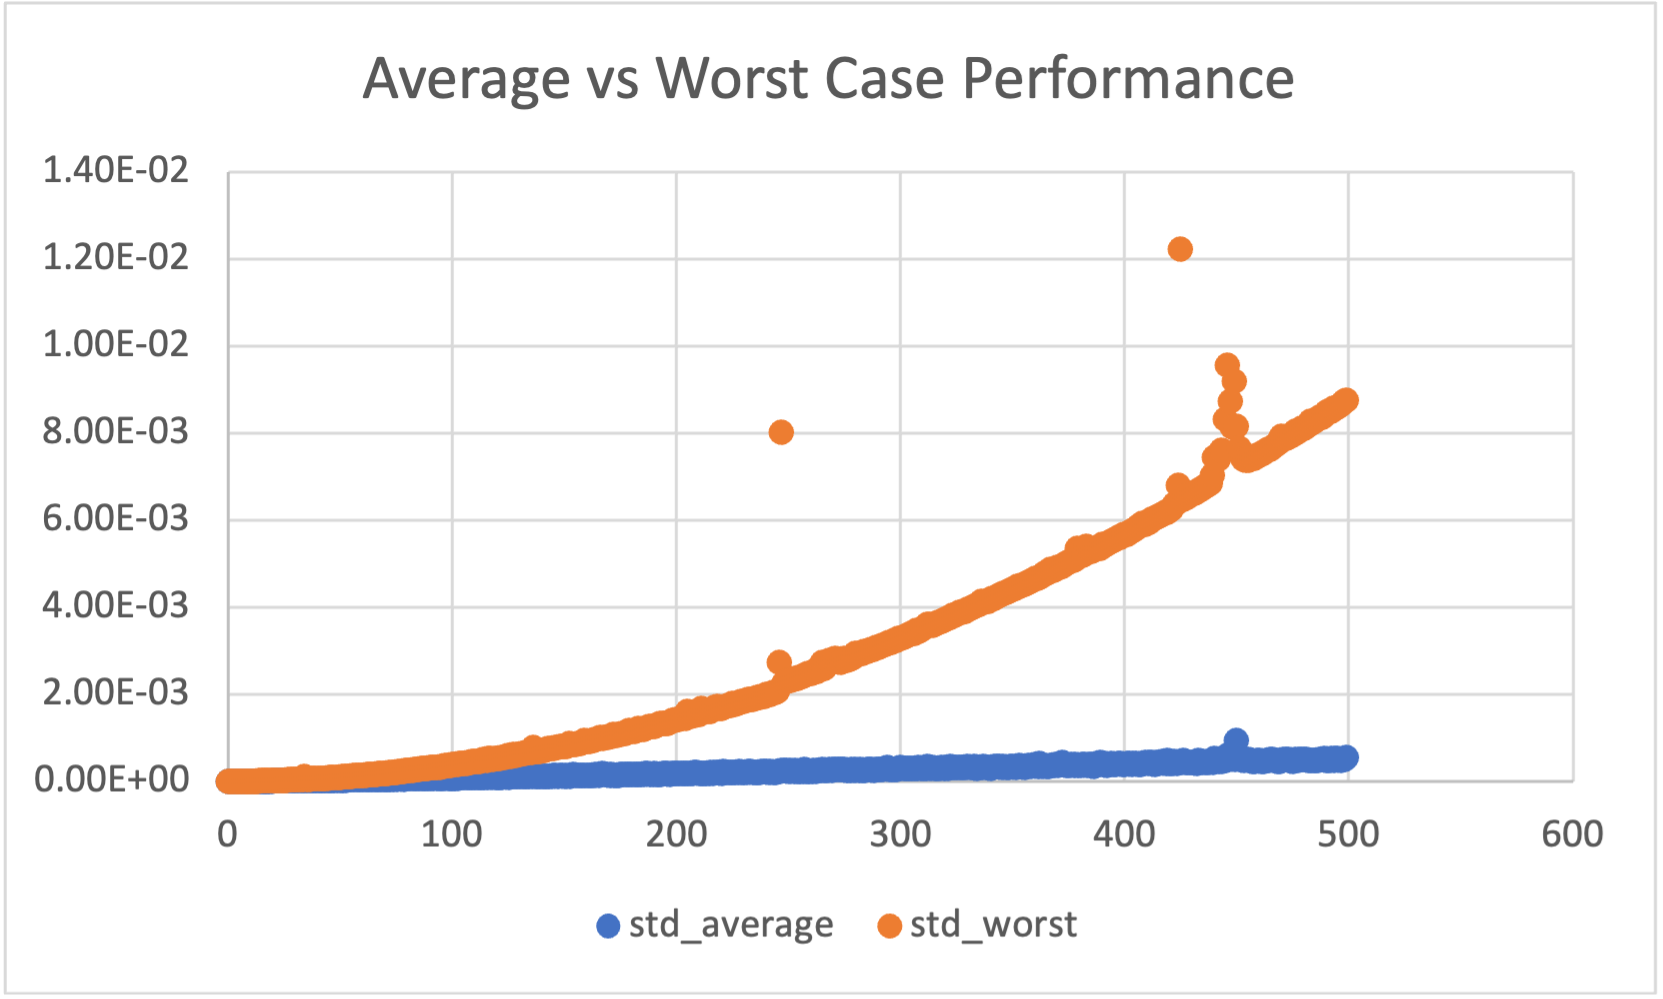
\includegraphics[width=0.8\textwidth]{average_vs_worst_case_performance}

\medskip
The function \verb|create_near_sorted_list| creates near-sorted-list based off 
some input factor. The lower the factor, the closer to being sorted the created list is.

Bubble sort will out-perform quicksort when a given list is close to being sorted 
since it only takes one or few iterations for the bubble sort to terminate, yielding 
a linear complexity($\Theta{n}$). Attached is a graph comparing their performance 
with factor ranging from 0 to 0.99. Note that the lists sorted are of length 996 
instead of 1000 as specified since it would otherwise generate \verb|RecursionError|.

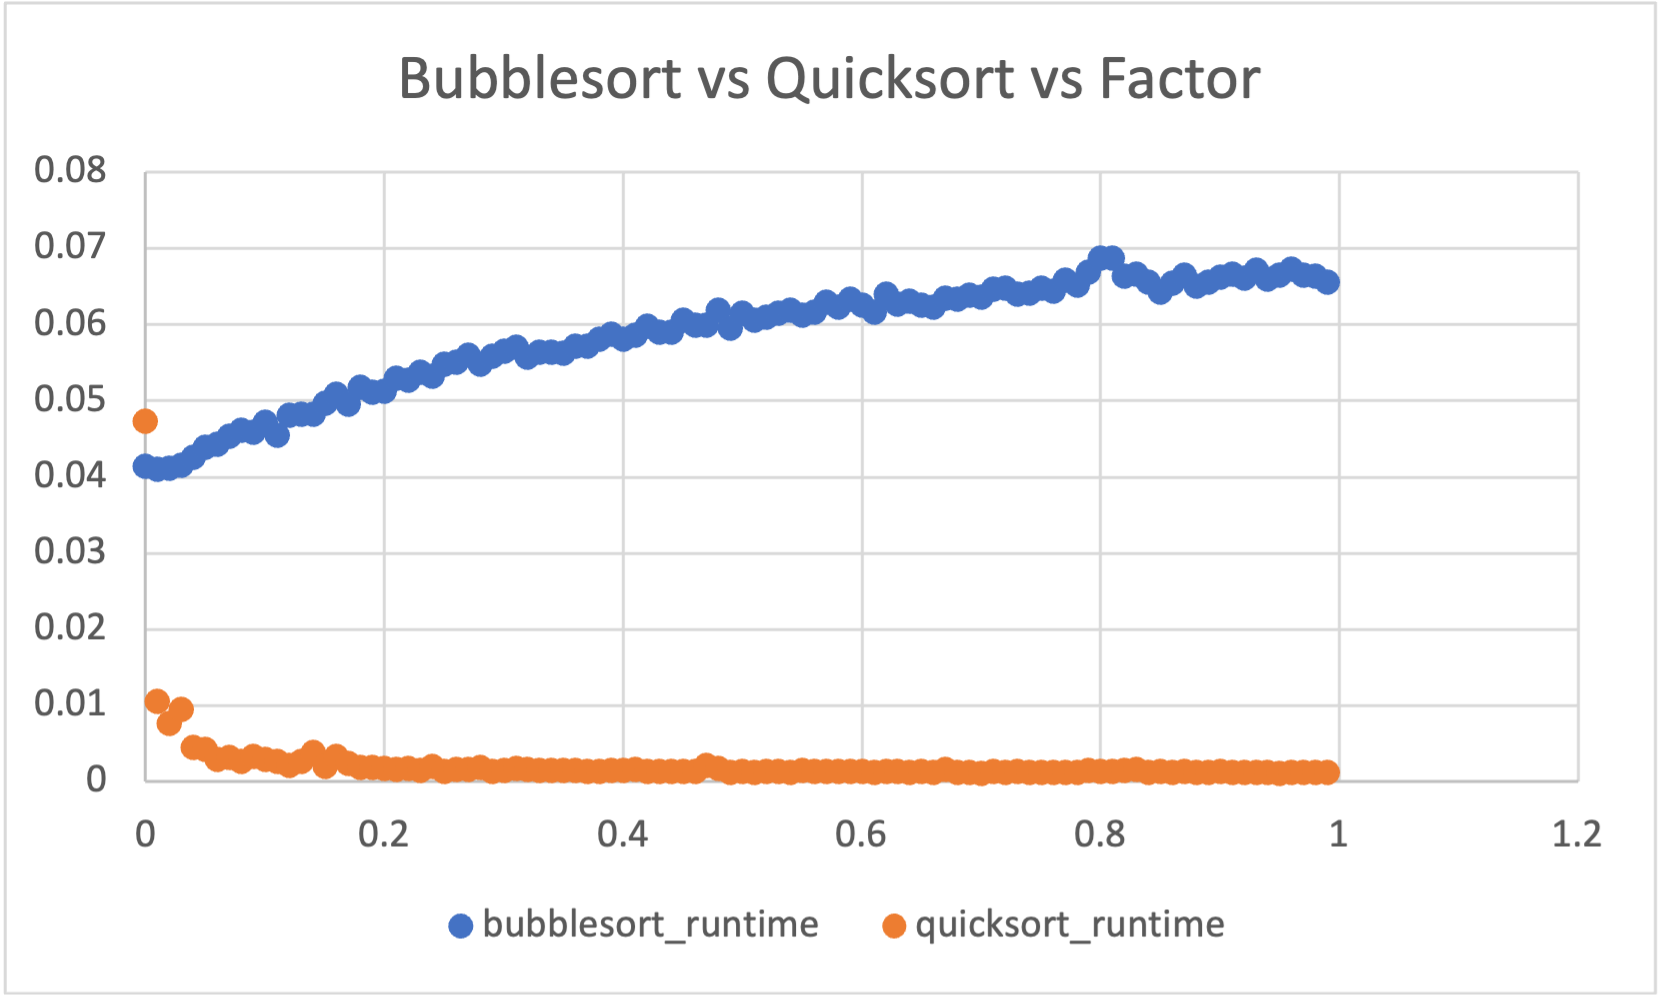
\includegraphics[width=0.8\textwidth]{bubblesort_vs_quicksort_vs_factor}

Bubble sort out-performs only when factor is extremely close to zero.

\medskip
Selection sort always has a complexity of $n^2$. Attached is a graph comparing their 
performance with factor ranging from 0 to 0.99. Note that the lists sorted are of 
length 996 instead of 1000 as specified since it would otherwise generate \verb|RecursionError|.

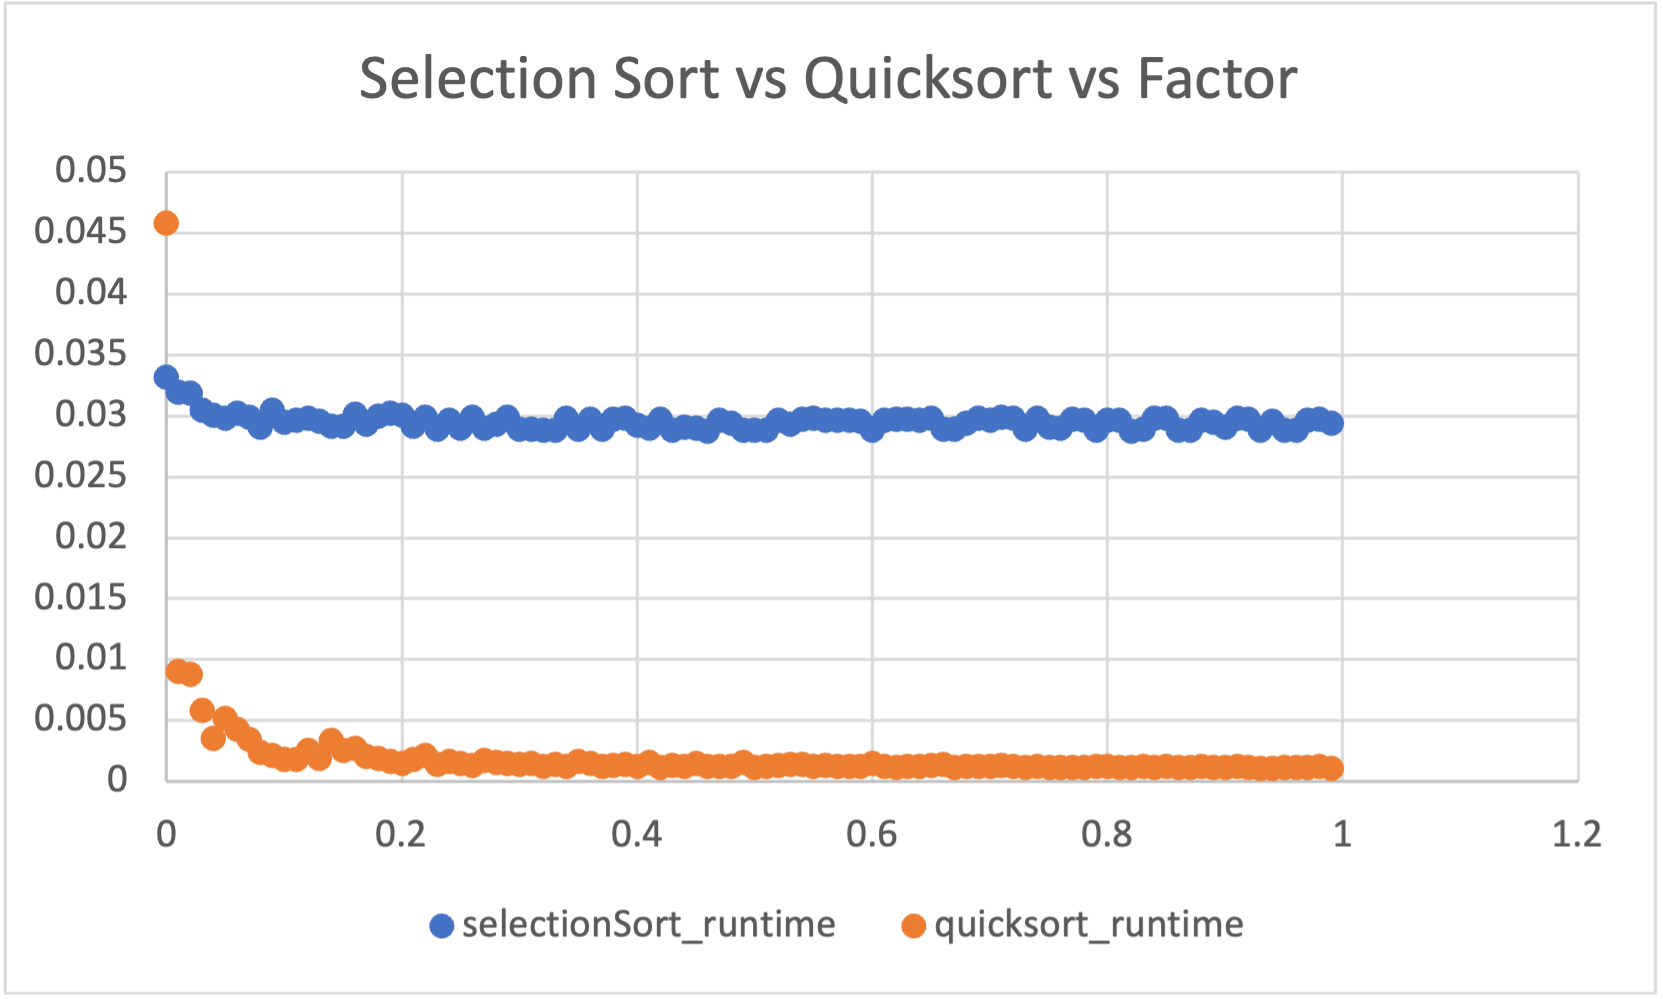
\includegraphics[width=0.8\textwidth]{selectionSort_vs_quicksort_vs_factor}

Selection sort out-performs only when factor is extremely close to zero.

\medskip
Insertion sort will out-perform quicksort when a given list is close to being sorted, 
yielding a linear complexity($\Theta{n}$). Attached is a graph comparing their 
performance with factor ranging from 0 to 0.99. Note that the lists sorted are of 
length 996 instead of 1000 as specified since it would otherwise generate \verb|RecursionError|.

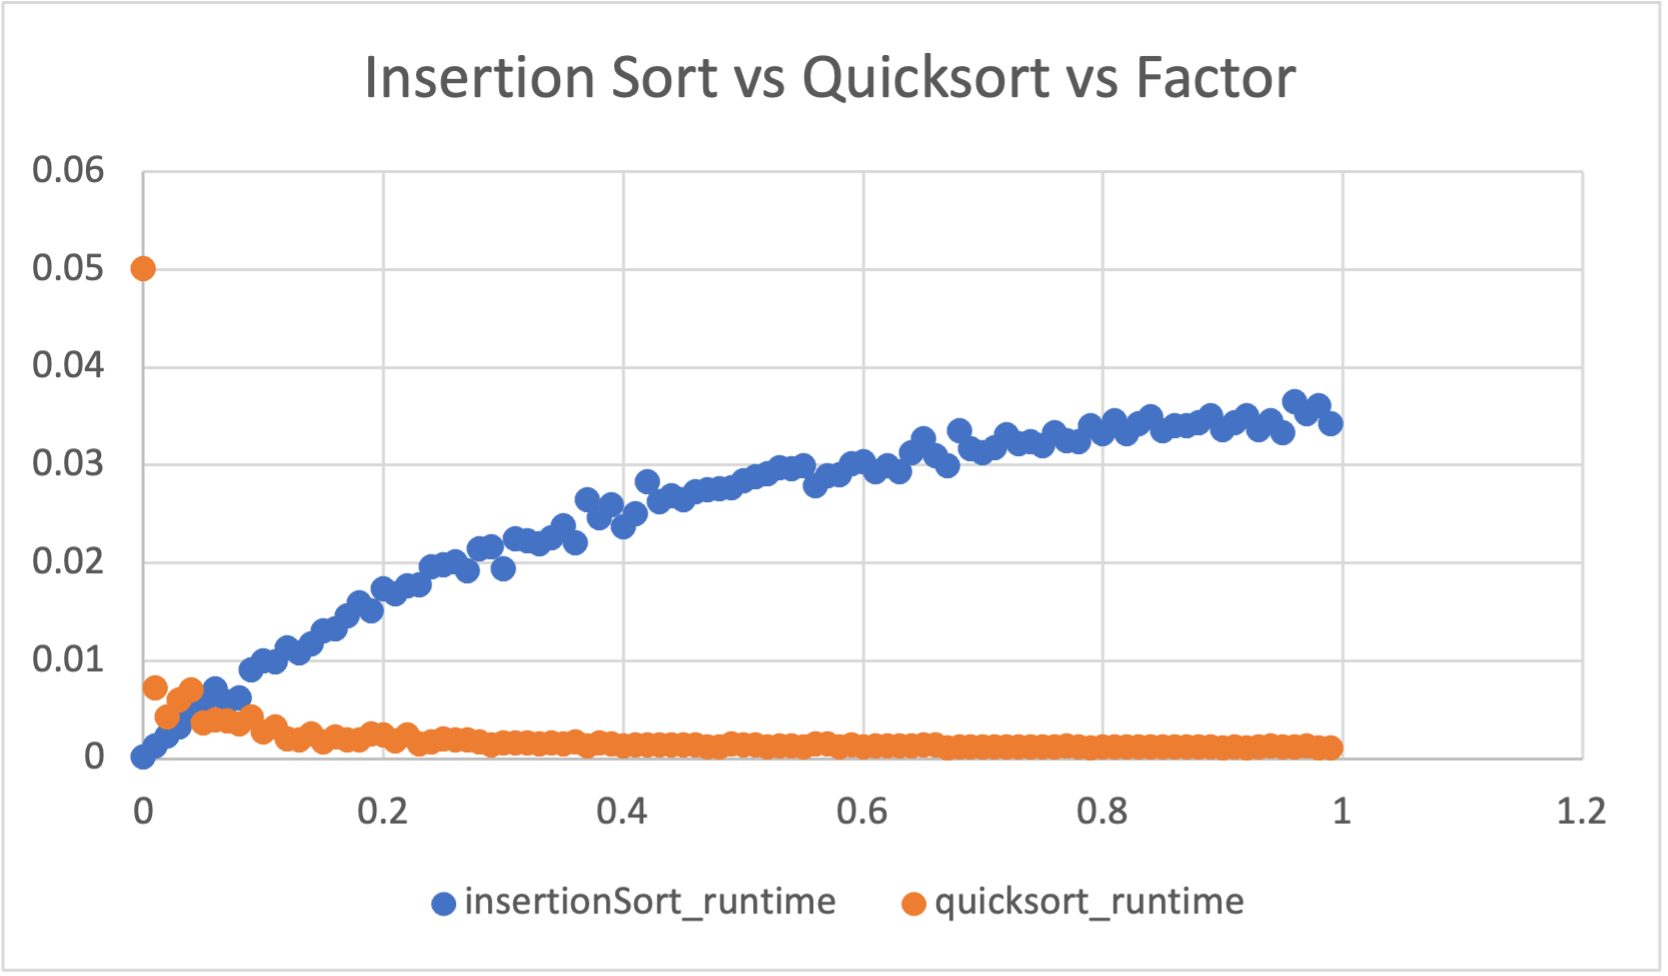
\includegraphics[width=0.8\textwidth]{insertionSort_vs_quicksort_vs_factor}

Insertion sort out-performs when factor approximately is smaller than 0.05.

\section*{Small lists}

\end{document}
